\documentclass[12pt]{article}
\usepackage[utf8]{inputenc}
\usepackage{float}
\usepackage{amsmath}


\usepackage[hmargin=3cm,vmargin=6.0cm]{geometry}
%\topmargin=0cm
\topmargin=-2cm
\addtolength{\textheight}{6.5cm}
\addtolength{\textwidth}{2.0cm}
%\setlength{\leftmargin}{-5cm}
\setlength{\oddsidemargin}{0.0cm}
\setlength{\evensidemargin}{0.0cm}

%misc libraries goes here
\usepackage{tikz}


\begin{document}

\section*{Student Information } 
%Write your full name and id number between the colon and newline
%Put one empty space character after colon and before newline
Full Name : Mustafa Sezgin \\
Id Number : 2380863 \\

% Write your answers below the section tags
\section*{Answer 1}

\subsection*{a)}
\begin{figure}[H]
    \centering
    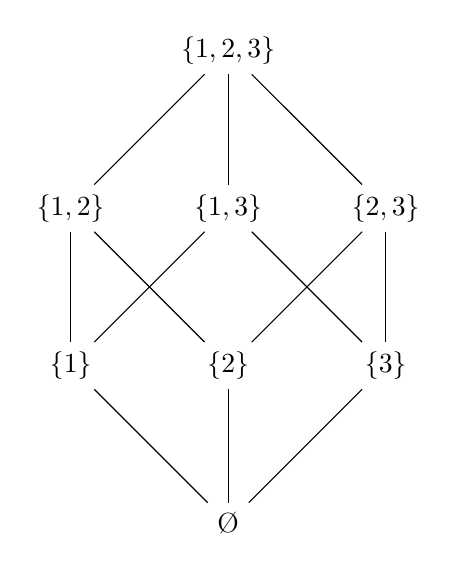
\begin{tikzpicture}
    
    \node (a) at (0,6)    {$\{1, 2, 3\}$};
    \node (b) at (-2,4)   {$\{1, 2\}$};
    \node (c) at (0,4)    {$\{1, 3\}$};
    \node (d) at (2,4)    {$\{2, 3\}$};
    \node (e) at (-2,2)   {$\{1\}$};
    \node (f) at (0,2)    {$\{2\}$};
    \node (g) at (2,2)    {$\{3\}$};
    \node (h) at (0,0)    {\O};
    
    \path[-] (a) edge (b);
    \path[-] (a) edge (c);
    \path[-] (a) edge (d);
    \path[-] (b) edge (e);
    \path[-] (b) edge (f);
    \path[-] (c) edge (e);
    \path[-] (c) edge (g);
    \path[-] (d) edge (f);
    \path[-] (d) edge (g);
    \path[-] (e) edge (h);
    \path[-] (f) edge (h);
    \path[-] (g) edge (h);
    
    \end{tikzpicture}
    \caption{Hasse Diagram}
    \label{fig:hasse}
\end{figure}

\subsection*{b)}
Yes. Every pair of elements has both a least upper bound and a greatest lower bound.

\subsection*{c)}
$\{1, 2, 3\}$

\subsection*{d)}
\O

\subsection*{e)}
Yes, $\{1, 2, 3\}$.

\subsection*{f)}
Yes, \O.

\subsection*{f)}
$\{1, 3\}$

\section*{Answer 2}

\subsection*{a)}
$2 \times 7 = 14$, by \textit{Handshaking Theorem}.

\subsection*{b)}
$14$. An edge occurs at both $ij$-th and $ji$-th entries in the matrix, since the graph is undirected.

\subsection*{c)}
$14$. It is equal to the sum of degrees of all nodes since two vertices are incident to each edge.

\subsection*{d)}
Yes.
\begin{figure}[H]
    \centering
    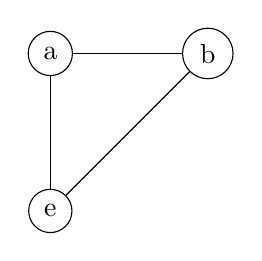
\begin{tikzpicture}
    
    \node[shape=circle, draw=black] (a) at (0, 2)   {a};
    \node[shape=circle, draw=black] (b) at (2, 2)   {b};
    \node[shape=circle, draw=black] (e) at (0, 0)   {e};
    
    \path[-] (a) edge (b);
    \path[-] (b) edge (e);
    \path[-] (e) edge (a);
    
    \end{tikzpicture}
    \caption{Complete Subgraph of $G$}
    \label{fig:complete}
\end{figure}

\subsection*{e)}
No. The subgraph obtained from $G$ by removing edges $(b, e)$ and $(c, d)$ is bipartite graph.

\subsection*{f)}
It is $2^7 = 128$, since each edge can have two different directions.

\subsection*{g)}
It is 7. The longest simple path is $[e, b, a, e, d, b, c, d]$.

\subsection*{h)}
It is 1. $G$ itself is a connected graph since every connected subgraph of it is a proper subgraph of another connected subgraph of it.

\subsection*{i)}
No. Since vertices $d$ and $e$ has odd degree, all vertices do not have even degree.

\subsection*{j)}
Yes. $[e, b, a, e, d, b, c, d]$ is an Euler Path, which is a simple path containing every edge exactly once.

\subsection*{k)}
Yes. $[a, b, c, d, e, a]$ is a Hamilton Circuit, which is a simple circuit containing every vertex except the starting one exactly once.

\subsection*{l)}
Yes. $[a, b, c, d, e]$ is a Hamilton path, which is a simple path containing every vertex exactly once.

\section*{Answer 3}
$G$ and $H$ are isomorphic. Both graphs have 8 vertices each of degree 4, and 16 edges. The function $f$ with $f(a) = a'$, $f(b) = c'$, $f(c) = e'$, $f(d) = g'$, $f(e) = b'$, $f(f) = h'$, $f(g) = d'$, and $f(h) = f'$ is a one-to-one correspondence between between the vertex set of $G$ and the vertex set of $H$. Also, for example, the simple circuit $[a, b, c, d, h, g, f, e, a]$ in $G$ is correspondent to the simple circuit $[a', c', e', g', f', d', h', b', a']$ in $H$, and the simple circuit $[a, e, b, g, c, h, d, f, a]$ in $G$ is correspondent to the simple circuit $[a', b', c', d', e', f', g', h', a']$ in $H$, and so on.

\section*{Answer 4}
Initially, path length to $a$ is 0, and to the rest is infinity. $S$ is empty. While $j$ is not in $S$, we will set $u$ as the unvisited vertex with the smallest path, add it to $S$, set it as visited, and update the path lengths and paths of its unvisited adjacents if necessary.

\begin{center}
\begin{tabular}{c|c|l|c}
    Vertex & Path Length & Path & Visited \\
    \hline
    a & 0 & [a] & \\
    b & $\infty$ & & \\
    c & $\infty$ & & \\
    d & $\infty$ & & \\
    e & $\infty$ & & \\
    f & $\infty$ & & \\
    g & $\infty$ & & \\
    h & $\infty$ & & \\
    i & $\infty$ & & \\
    j & $\infty$ & & \\
    k & $\infty$ & &
\end{tabular}
\end{center}

$j \notin S = \{\}$ \\
$u = a$, $S = \{a\}$ \\
$L(a) + w(a, b) = 0 + 3 = 3 < \infty$, then $L(b) = 3$ \\
$L(a) + w(a, e) = 0 + 5 = 5 < \infty$, then $L(e) = 5$ \\
$L(a) + w(a, h) = 0 + 4 = 4 < \infty$, then $L(h) = 4$ \\

\begin{center}
\begin{tabular}{c|c|l|c}
    Vertex & Path Length & Path & Visited \\
    \hline
    a & 0 & [a] & + \\
    b & 3 & [a, b] & \\
    c & $\infty$ & & \\
    d & $\infty$ & & \\
    e & 5 & [a, e] & \\
    f & $\infty$ & & \\
    g & $\infty$ & & \\
    h & 4 & [a, h] & \\
    i & $\infty$ & & \\
    j & $\infty$ & & \\
    k & $\infty$ & &
\end{tabular}
\end{center}

$j \notin S = \{a\}$ \\
$u = b$, $S = \{a, b\}$ \\
$L(b) + w(b, c) = 3 + 2 = 5 < \infty$, then $L(c) = 5$ \\
$L(b) + w(b, e) = 3 + 5 = 8 \not< 5$ \\
$L(b) + w(b, f) = 3 + 7 = 10 < \infty$, then $L(f) = 10$ \\

\begin{center}
\begin{tabular}{c|c|l|c}
    Vertex & Path Length & Path & Visited \\
    \hline
    a & 0 & [a] & + \\
    b & 3 & [a, b] & + \\
    c & 5 & [a, b, c] & \\
    d & $\infty$ & & \\
    e & 5 & [a, e] & \\
    f & 10 & [a, b, f] & \\
    g & $\infty$ & & \\
    h & 4 & [a, h] & \\
    i & $\infty$ & & \\
    j & $\infty$ & & \\
    k & $\infty$ & &
\end{tabular}
\end{center}

$j \notin S = \{a, b\}$ \\
$u = h$, $S = \{a, b, h\}$ \\
$L(h) + w(h, e) = 4 + 7 = 11 \not< 5$ \\
$L(h) + w(h, f) = 4 + 5 = 9 < 10$, then $L(f) = 9$ \\
$L(h) + w(h, i) = 4 + 2 = 6 < \infty$, then $L(i) = 6$ \\

\begin{center}
\begin{tabular}{c|c|l|c}
    Vertex & Path Length & Path & Visited \\
    \hline
    a & 0 & [a] & + \\
    b & 3 & [a, b] & + \\
    c & 5 & [a, b, c] & \\
    d & $\infty$ & & \\
    e & 5 & [a, e] & \\
    f & 9 & [a, h, f] & \\
    g & $\infty$ & & \\
    h & 4 & [a, h] & + \\
    i & 6 & [a, h, i] & \\
    j & $\infty$ & & \\
    k & $\infty$ & &
\end{tabular}
\end{center}

$j \notin S = \{a, b, h\}$ \\
$u = c$, $S = \{a, b, h, c\}$ \\
$L(c) + w(c, d) = 5 + 3 = 8 < \infty$, then $L(d) = 8$ \\
$L(c) + w(c, f) = 5 + 2 = 7 < 9$, then $L(f) = 7$ \\
$L(c) + w(c, g) = 5 + 6 = 11 < \infty$, then $L(g) = 11$ \\

\begin{center}
\begin{tabular}{c|c|l|c}
    Vertex & Path Length & Path & Visited \\
    \hline
    a & 0 & [a] & + \\
    b & 3 & [a, b] & + \\
    c & 5 & [a, b, c] & + \\
    d & 8 & [a, b, c, d] & \\
    e & 5 & [a, e] & \\
    f & 7 & [a, b, c, f] & \\
    g & 11 & [a, b, c, g] & \\
    h & 4 & [a, h] & + \\
    i & 6 & [a, h, i] & \\
    j & $\infty$ & & \\
    k & $\infty$ & &
\end{tabular}
\end{center}

$j \notin S = \{a, b, h, c\}$ \\
$u = e$, $S = \{a, b, h, c, e\}$ \\
$L(e) + w(e, f) = 5 + 4 = 9 \not< 7$ \\

\begin{center}
\begin{tabular}{c|c|l|c}
    Vertex & Path Length & Path & Visited \\
    \hline
    a & 0 & [a] & + \\
    b & 3 & [a, b] & + \\
    c & 5 & [a, b, c] & + \\
    d & 8 & [a, b, c, d] & \\
    e & 5 & [a, e] & + \\
    f & 7 & [a, b, c, f] & \\
    g & 11 & [a, b, c, g] & \\
    h & 4 & [a, h] & + \\
    i & 6 & [a, h, i] & \\
    j & $\infty$ & & \\
    k & $\infty$ & &
\end{tabular}
\end{center}

$j \notin S = \{a, b, h, c, e\}$ \\
$u = i$, $S = \{a, b, h, c, e, i\}$ \\
$L(i) + w(i, f) = 6 + 4 = 10 \not< 7$ \\
$L(i) + w(i, j) = 6 + 6 = 12 < \infty$, then $L(j) = 12$ \\

\begin{center}
\begin{tabular}{c|c|l|c}
    Vertex & Path Length & Path & Visited \\
    \hline
    a & 0 & [a] & + \\
    b & 3 & [a, b] & + \\
    c & 5 & [a, b, c] & + \\
    d & 8 & [a, b, c, d] & \\
    e & 5 & [a, e] & + \\
    f & 7 & [a, b, c, f] & \\
    g & 11 & [a, b, c, g] & \\
    h & 4 & [a, h] & + \\
    i & 6 & [a, h, i] & + \\
    j & 12 & [a, h, i, j] & \\
    k & $\infty$ & &
\end{tabular}
\end{center}

$j \notin S = \{a, b, h, c, e, i\}$ \\
$u = f$, $S = \{a, b, h, c, e, i, f\}$ \\
$L(f) + w(f, g) = 7 + 4 = 11 \not< 11$ \\
$L(f) + w(f, j) = 7 + 3 = 10 < 12$, then $L(j) = 10$ \\

\begin{center}
\begin{tabular}{c|c|l|c}
    Vertex & Path Length & Path & Visited \\
    \hline
    a & 0 & [a] & + \\
    b & 3 & [a, b] & + \\
    c & 5 & [a, b, c] & + \\
    d & 8 & [a, b, c, d] & \\
    e & 5 & [a, e] & + \\
    f & 7 & [a, b, c, f] & + \\
    g & 11 & [a, b, c, g] & \\
    h & 4 & [a, h] & + \\
    i & 6 & [a, h, i] & + \\
    j & 10 & [a, b, c, f, j] & \\
    k & $\infty$ & &
\end{tabular}
\end{center}

$j \notin S = \{a, b, h, c, e, i, f\}$ \\
$u = d$, $S = \{a, b, h, c, e, i, f, d\}$ \\
$L(d) + w(d, g) = 8 + 7 = 15 \not< 11$ \\
$L(d) + w(d, k) = 8 + 2 = 10 < \infty$, then $L(k) = 10$ \\

\begin{center}
\begin{tabular}{c|c|l|c}
    Vertex & Path Length & Path & Visited \\
    \hline
    a & 0 & [a] & + \\
    b & 3 & [a, b] & + \\
    c & 5 & [a, b, c] & + \\
    d & 8 & [a, b, c, d] & + \\
    e & 5 & [a, e] & + \\
    f & 7 & [a, b, c, f] & + \\
    g & 11 & [a, b, c, g] & \\
    h & 4 & [a, h] & + \\
    i & 6 & [a, h, i] & + \\
    j & 10 & [a, b, c, f, j] & \\
    k & 10 & [a, b, c, d, k] &
\end{tabular}
\end{center}

$j \notin S = \{a, b, h, c, e, i, f, d\}$ \\
$u = j$, $S = \{a, b, h, c, e, i, f, d, j\}$ \\
$L(j) + w(j, g) = 10 + 4 = 14 \not< 11$ \\
$L(j) + w(j, k) = 10 + 2 = 12 \not< 10$ \\

\begin{center}
\begin{tabular}{c|c|l|c}
    Vertex & Path Length & Path & Visited \\
    \hline
    a & 0 & [a] & + \\
    b & 3 & [a, b] & + \\
    c & 5 & [a, b, c] & + \\
    d & 8 & [a, b, c, d] & + \\
    e & 5 & [a, e] & + \\
    f & 7 & [a, b, c, f] & + \\
    g & 11 & [a, b, c, g] & \\
    h & 4 & [a, h] & + \\
    i & 6 & [a, h, i] & + \\
    j & 10 & [a, b, c, f, j] & + \\
    k & 10 & [a, b, c, d, k] &
\end{tabular}
\end{center}

$j \in S = \{a, b, h, c, e, i, f, d, j\}$, loop terminates. The shortest path from $a$ to $j$ is $[a, b, c, f, j]$ with length 10.

\section*{Answer 5}

\subsection*{a)}
By Prim's algorithm, edges added to the tree are $(a, b)$, $(a, d)$, $(b, c)$, $(c, e)$, and $(e, f)$ respectively.

\subsection*{b)}
\begin{figure}[H]
	\centering
	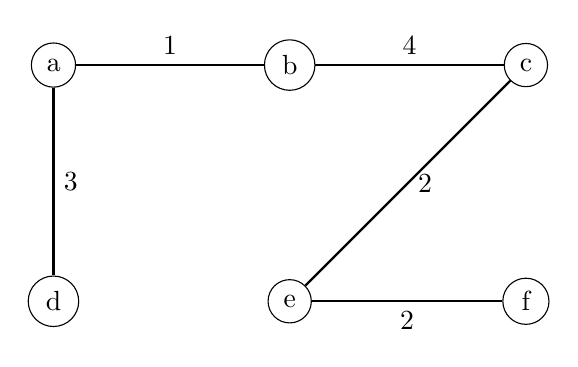
\begin{tikzpicture}
	
	\node[shape=circle,draw=black] (a) at (0, 3)     {a};
	\node[shape=circle,draw=black] (b) at (3, 3)     {b};
	\node[shape=circle,draw=black] (c) at (6, 3)     {c};
	\node[shape=circle,draw=black] (d) at (0, 0)     {d};
	\node[shape=circle,draw=black] (e) at (3, 0)     {e};
	\node[shape=circle,draw=black] (f) at (6, 0)     {f};
	
	\path[-, thick] (a) edge node[above]{1} (b);
	\path[-, thick] (b) edge node[above]{4} (c);
	\path[-, thick] (a) edge node[right]{3} (d);
	\path[-, thick] (c) edge node[right]{2} (e);
	\path[-, thick] (e) edge node[below]{2} (f);
	
	\end{tikzpicture} 
	\caption{Minimum Spanning Tree for $G$}
	\label{fig:minspantree}
\end{figure}

\subsection*{c)}
No. There are three edges with length 2 that form a circuit. We can choose to remove any of them while constructing the minimum spanning tree. Therefore, the tree is not unique.

\section*{Answer 6}

\subsection*{a)}
There are 13 vertices, 12 edges, and the height of $T$ is 4.

\subsection*{b)}
$[w, s, m, t, q, x, n, y, u, z, v, r, p]$

\subsection*{c)}
$[s, w, q, m, t, p, x, u, n, y, r, v, z]$

\subsection*{d)}
$[p, q, s, w, t, m, r, u, x, y, n, v, z]$

\subsection*{e)}
No. Some internal vertices have one child instead of two.

\end{document}